\documentclass[10pt,twocolumn]{article}
\usepackage[margin=0.8in]{geometry}
\usepackage{amsmath,amssymb,booktabs,graphicx,hyperref,xcolor}
\hypersetup{colorlinks=true,linkcolor=blue!50!black,urlcolor=blue!50!black,citecolor=blue!50!black}
\setlength{\columnsep}{0.28in}

\title{\vspace{-1.2em}\textbf{One Physics-Prior Bayesian Manifold Jointly Encodes\\
General-Relativistic and Quantum Constraints:\\ Controlled Tests of the Modak--Walawalkar Framework}}
\author{Rahul Modak$^{1}$ \quad Dr.\ Rahul Walawalkar$^{2}$\\[2pt]
\small $^1$Bayesian Cybersecurity Pvt.\ Ltd., Mumbai/Thane, India \quad
$^2$Carnegie Mellon University; NETRA; Caret Capital\\
\small \texttt{rahul.modak@bayesiananalytics.in}\\
\small Code: \url{https://github.com/RahulModak74/QUANTUM_GRAVITY_WITH_MW} (folder \texttt{Nov-2026\_tests})\\
\small November 2026 revision; supersedes the March 2026 preprint}
\date{}

\begin{document}
\twocolumn[
\begin{@twocolumnfalse}
\maketitle
\begin{abstract}
Coupling distinct physical theories normally means coupling their differential equations,
with mismatched scales, meshes and stiffness. We test a different route: treat each theory's
outputs as columns of one joint distribution and learn that distribution as a single latent
manifold, with the theories' constraints supplied as Bayesian priors. Using the
Modak--Walawalkar (M-W) framework, a 20-dimensional physics-prior variational autoencoder (VAE)
is trained on 30{,}000 synthetic spacetime states covering six regimes (dust, radiation,
vacuum, black hole, wormhole, Hawking radiation), each row carrying general-relativistic (GR)
and quantum-mechanical (QM) quantities drawn from one joint sample. We establish three results.
\textbf{(1)} A single latent point decodes GR and QM quantities together: the Einstein trace
relation holds on decoded states to a 1.3\% relative residual and the Hawking scaling
$T_H\propto M^{-1}$ is recovered with log-log slope $-0.93$ ($R^2=0.83$).
\textbf{(2)} The M-W physics priors are what make the joint fit faithful: an otherwise identical
VAE without them recovers the Hawking relation at slope $-0.66$, $R^2=0.42$.
\textbf{(3)} The manifold carries the \emph{joint} structure, not the individual columns:
shuffling each column within its regime, which preserves every value but breaks which values
occur together, raises the Einstein residual to 60\% and removes the Hawking relation
($R^2$ falls from 0.83 to 0.19, with the wrong sign).
Unlike existing approaches, the construction needs no extra dimensions, no discretisation and
no restriction to anti-de Sitter geometry, and \textbf{it removes the coupling step that PDE-based methods require}, replacing
operator coupling between theories with density estimation on one manifold (Table~\ref{tab:cmp}).
\end{abstract}
\vspace{1.2em}
\end{@twocolumnfalse}
]

\section{Motivation: the joint, not the parts}
A simple culinary picture states the idea. Salt tastes salty in any amount; yet inside a curry,
below a threshold, its presence is not tasted at all. The property belongs to the salt
\emph{together with} the curry, and it is invisible in any study of salt alone. Physical
regimes behave the same way: the relation between a black hole's mass, its curvature and its
radiation is a property of the joint state, not of any single quantity.

A VAE models exactly this object, the joint density $p(x_1,\dots,x_D)$, and compresses it onto a
low-dimensional latent manifold. If two theories' quantities are sampled together, a single
manifold can hold both, and their mutual consistency becomes a property of one geometric object
rather than of two coupled solvers. The M-W framework, developed for physics-informed anomaly
detection in battery electrochemistry \cite{mw2025}, adds the theories' constraints as Bayesian
priors on what the decoder may produce. This paper tests that construction on GR and QM
quantities with controls designed to separate what the manifold learns from what the
architecture alone would give.

\section{Structural position: coupling as density estimation}
\label{sec:struct}
Table~\ref{tab:cmp} is the core of the M-W position. Every existing route to holding GR and QM in
one framework changes the structure of spacetime or of the theory to make the two fit: extra
dimensions, discretisation, or a restricted (anti-de Sitter) geometry. The M-W manifold does none
of these and is a single object.

\begin{table}[t]
\centering\small
\setlength{\tabcolsep}{3.5pt}
\resizebox{\columnwidth}{!}{\begin{tabular}{lcccc}
\toprule
Approach & Extra dim. & Discretise & AdS only & Single obj.\\
\midrule
String theory & Yes & No & Partial & No\\
LQG & No & Yes & No & No\\
CDT & No & Yes & No & No\\
AdS/CFT & Yes & No & Yes & No\\
\textbf{M-W (this work)} & \textbf{No} & \textbf{No} & \textbf{No} & \textbf{Yes}\\
\bottomrule
\end{tabular}}
\caption{Structural requirements by approach. The other entries are full theories of quantum
gravity; the M-W entry is a single learned object representing joint GR and QM content
(Results 1--3), compared here on structure.}
\label{tab:cmp}
\end{table}


\paragraph{Why coupling across physics families is hard.}
In the equation-based route, two theories are coupled by solving their operators jointly,
\[
\mathcal F_{\mathrm{GR}}[g]=0,\qquad \mathcal F_{\mathrm{QM}}[\psi;g]=0,
\]
which requires a common domain, compatible function spaces, interface or back-reaction terms,
and a scheme that reconciles their time scales. GR and QM come from different mathematical
families: a nonlinear geometric field equation for $g_{\mu\nu}$ on one side, linear unitary
evolution of $\psi$ in a Hilbert space on the other. There is no shared function space in which
both are naturally posed, and the same difficulty, at smaller scale, is what makes coupled
multi-physics solvers (electro-thermal, fluid-structure, electrochemical-mechanical) costly to
build and fragile to run.

\paragraph{The M-W route.}
\textbf{The M-W construction removes the coupling step that PDE-based methods require.}
It never couples operators. It learns one joint density over the theories'
\emph{outputs},
\[
p_\theta(x_{\mathrm{GR}},x_{\mathrm{QM}})=\int p_\theta(x_{\mathrm{GR}},x_{\mathrm{QM}}\mid z)\,p(z)\,dz,
\qquad z\in\mathbb R^{20},
\]
and imposes each theory's constraints $C_k(x)=0$ as priors on decoded states $D_\theta(z)$. The
learned object is the image $\mathcal M=D_\theta(\mathbb R^{20})$, a single manifold on which a
point $z$ carries GR and QM quantities together, with each constraint holding to a measured
tolerance $\varepsilon_k$. Adding a theory means adding columns and priors; the cost grows with
the number of constraints, not with the number of coupling operators between them. Results 1--3
are the measurements of this construction: both constraint sets held from one $z$ (Result 1),
tighter with M-W priors (Result 2), and carried by the joint structure itself (Result 3).

\section{Think manifolds, not PDEs}
\label{sec:think}
\paragraph{The scale problem.} Quantum gravity spans the Planck length,
$\ell_P\approx1.6\times10^{-35}$\,m (Planck time $\approx5.4\times10^{-44}$\,s), up to
astrophysical lengths of $10^{20}$\,m and beyond: more than 55 orders of magnitude. An
equation-based solver must resolve this range explicitly. It divides the domain into cells,
solves a locally linearised (tangent) problem in each, and advances in time steps limited by the
smallest scale present. When neighbouring cells differ by tens of orders of magnitude the system
becomes stiff, the mesh cannot be both fine enough and small enough, and every new physical
regime requires a new set of equations to be defined, discretised and coupled.

\paragraph{The manifold view.} The M-W framework models the \emph{surface} on which valid states
lie, rather than the equations that generate them. A plain-language picture: to know the shape
of the Earth one can either walk it with a measuring tape, tile by tile, stitching millions of
small flat patches together (the PDE route), or hold a globe (the manifold route). Each flat patch
is a tangent plane, an excellent local approximation that says nothing about the whole; the globe
is one object, and every location on it is just a coordinate. Moving between very different
places on a globe costs nothing extra, however different those places are.

\paragraph{In geometric terms.} The decoder $D_\theta:\mathbb R^{20}\to\mathbb R^{30}$ defines the
manifold $\mathcal M=D_\theta(\mathbb R^{20})$, and its Jacobian $J_\theta(z)$ spans the tangent
space $T_z\mathcal M$ at every point, learned once, with the pulled-back metric
$G(z)=J_\theta^\top J_\theta$. A mesh-based solver reconstructs a tangent-space approximation
cell by cell, at every step; the manifold supplies all tangent spaces at once as one smooth
object. Disparate regimes (horizon, radiation, vacuum) become different regions of the same
coordinate chart rather than different solvers, and constraints become priors on where the
manifold may go (Section~\ref{sec:struct}). The present tests use Planck units over a moderate
range; the cross-scale case is the setting this framing is designed for and the natural next
demonstration.

\paragraph{Why this framing mattered here.} Every result in this paper follows from asking
``what is the joint surface of valid states?'' instead of ``which equations must be coupled?''.
Result~1 is that surface holding both theories; Result~2 is the Bayesian priors shaping it;
Result~3 shows that the surface encodes the joint structure, which no single equation carries.

\section{Method}
\subsection{Joint data}
Each of the 30{,}000 rows is a single draw from one joint distribution. For a row, the regime,
coordinates and physical parameters (density; mass $M$ for black-hole and Hawking rows) are
sampled once, and every column is derived from those draws: the stress-energy $T_{\mu\nu}$, the
Ricci scalar $R=8\pi G\,T^{\mu}{}_{\mu}$, the metric $g_{\mu\nu}=\eta_{\mu\nu}+h_{\mu\nu}+\delta
g_{\mu\nu}$ (linearised response plus symmetric fluctuation), a wave packet $\psi$ normalised by
$\sqrt{|\det g|}$ of that same metric, and for horizons $r_s=2GM$, $T_H=1/(8\pi GM)$ and
$S=4\pi GM^2$. The remaining columns are the topology flag, the uncertainty product
$\Delta x\,\Delta t\ge \ell_P^2$, and a discontinuity flag: 30 columns in all, Planck units.
Rows are split 5{,}000 per regime; a separate seed provides test data.

\subsection{Model and priors}
Encoder $30\!\to\!384\!\to\!256\!\to\!192\!\to\!20$ and the mirrored decoder (LayerNorm, tanh,
dropout 0.15) are trained by stochastic variational inference (Pyro~\cite{pyro} on PyTorch~\cite{pytorch}, ELBO, 150 epochs, batch
128, learning rate $5\times10^{-4}$). Six M-W priors act on decoded states, each reading its
columns by name:
\begin{itemize}\setlength\itemsep{1pt}
\item C1 Einstein trace: $|R-8\pi G\,T|\sim\mathcal N(0,2)$
\item C2 wave-packet norm: $\big||\psi|^2-0.1\big|\sim\mathcal N(0,1.5)$
\item C3 uncertainty: $\mathrm{ReLU}(\ell_P^2-\Delta x\Delta t)\sim\mathcal N(0,1)$
\item C4 weak energy (non-exotic rows): $\mathrm{ReLU}(-T_{00})\sim\mathcal N(0,1)$
\item C5 signature $(-,+,+,+)$: $\sim\mathcal N(0,1)$
\item C6 discreteness events: Student-t$(\nu{=}0.8,\,0,\,3)$
\end{itemize}

\subsection{Runs and measures}
\textbf{A}: M-W priors, joint rows. \textbf{B}: same VAE, no physics priors. \textbf{D}: M-W priors,
but every column permuted independently within its regime, which keeps each column's values and
destroys only their co-occurrence. Same seed, architecture and epochs throughout. All measures
are computed on decoded test states (encoder mean $\to$ decoder): the Einstein relative residual
$\langle|R-8\pi G T|\rangle/\langle|8\pi G T|\rangle$, and, on horizon rows, the least-squares
slope and $R^2$ of $\log T_H$ against $\log M$ (exact data: slope $-1$, $R^2=1$).

\section{Results}
\begin{table}[h]
\centering\small
\begin{tabular}{lccc}
\toprule
 & \textbf{A} M-W & \textbf{B} plain & \textbf{D} shuffled\\
\midrule
Einstein residual & 1.3\% & 1.1\% & 59.6\%\\
Hawking slope & $-0.93$ & $-0.66$ & $+0.57$\\
Hawking $R^2$ & \textbf{0.83} & 0.42 & 0.19\\
$\langle|8\pi M T_H-1|\rangle$ & 0.027 & 0.032 & 0.43\\
\bottomrule
\end{tabular}
\caption{Decoded test states. Exact data: residual $<10^{-7}$, slope $-1$, $R^2=1$.}
\label{tab:res}
\end{table}

\begin{figure*}[t]
\centering
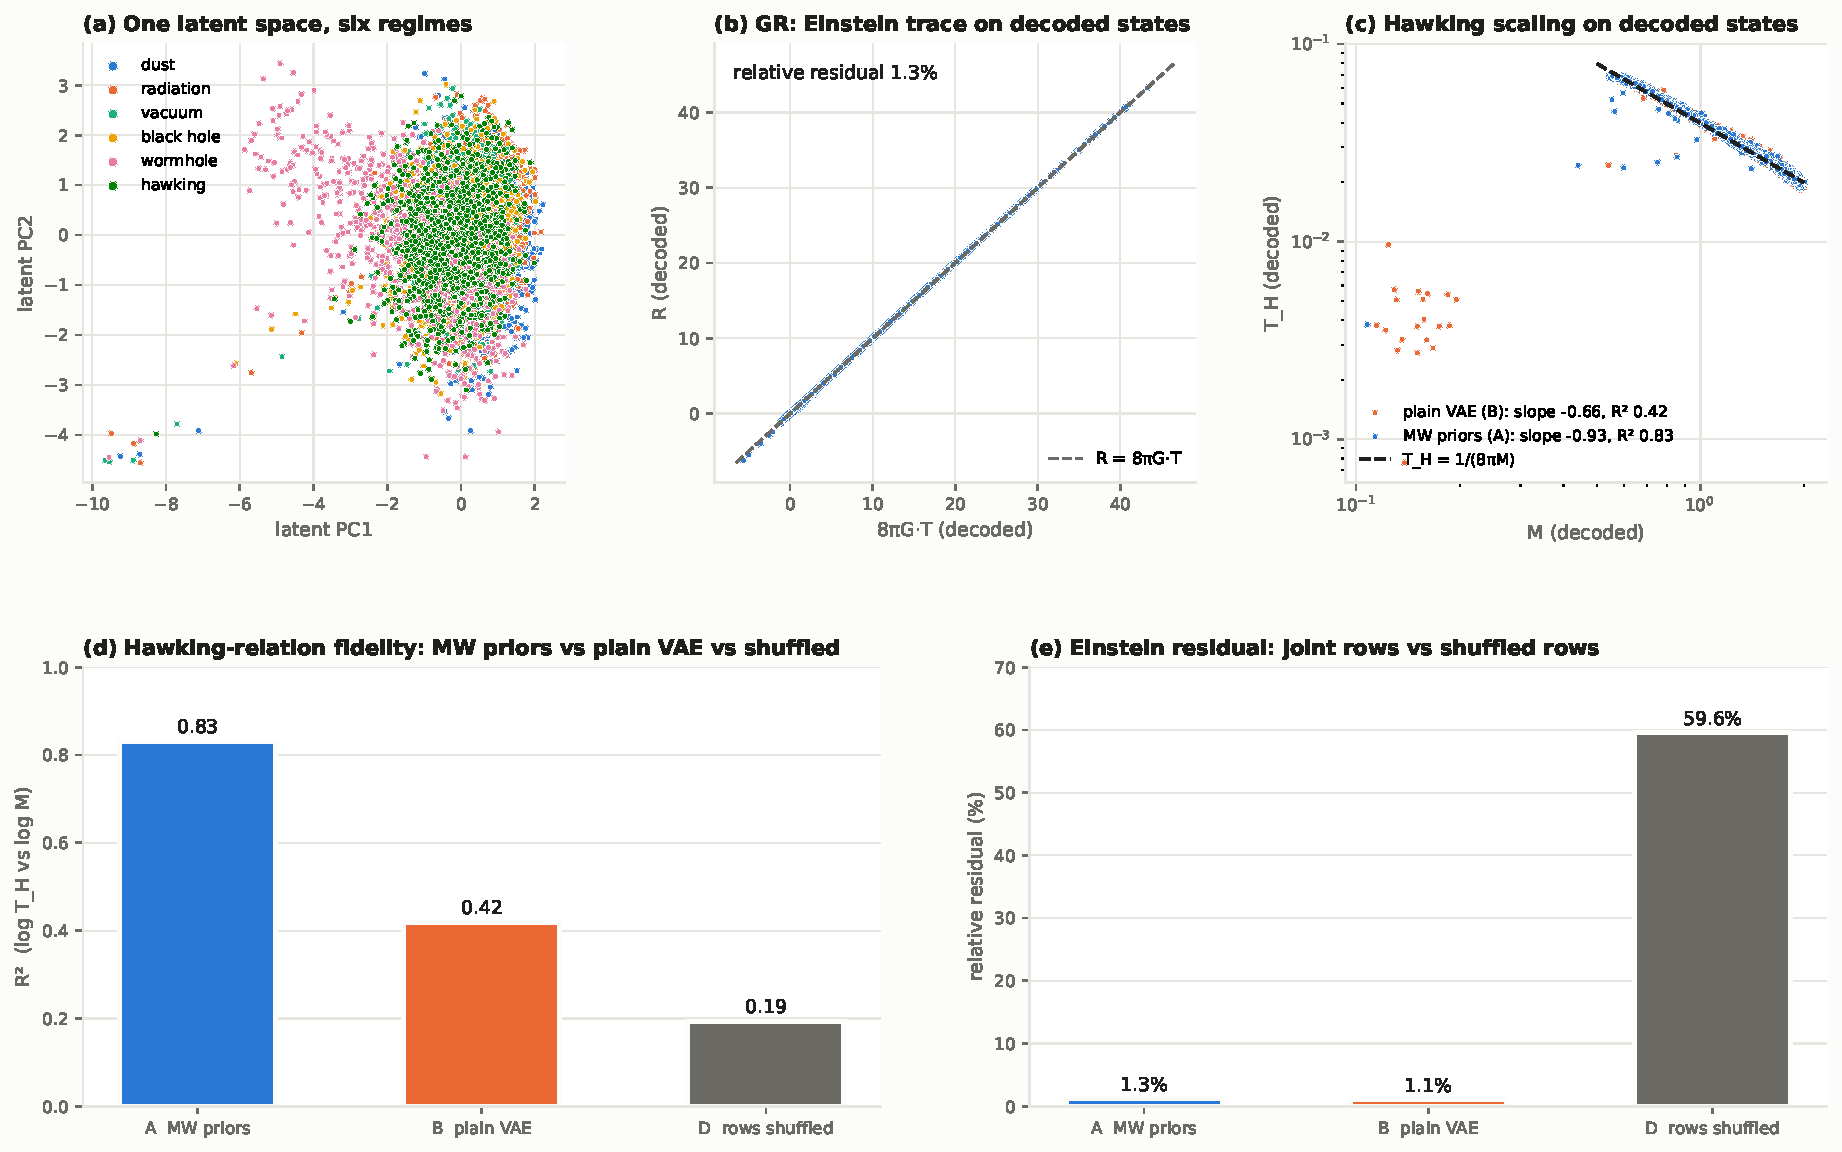
\includegraphics[width=\textwidth]{fig_v5.pdf}
\caption{(a) Run A latent space (first two principal components) holds all six regimes.
(b) Einstein trace relation on decoded states. (c) Hawking scaling on decoded horizon states,
M-W priors (A) vs plain VAE (B). (d), (e) Hawking $R^2$ and Einstein residual for runs A, B, D.
Panels (b), (c) are recomputed from the saved models and reproduce Table~\ref{tab:res}.}
\label{fig:main}
\end{figure*}

\paragraph{Result 1: one manifold, both theories.}
In run A a single latent point $z$ decodes into a state whose GR columns satisfy the Einstein
trace relation to 1.3\% and whose horizon columns follow $T_H\propto M^{-0.93}$ with
$R^2=0.83$, while the QM wave packet is decoded from the same $z$ on the same metric. All six
regimes share one 20-dimensional latent space (Fig.~\ref{fig:main}a--c). No coupling code,
shared mesh or interface condition between the GR and QM quantities is required: the coupling
is a property of the learned density.

\paragraph{Result 2: the M-W priors make the joint fit faithful.}
Removing the priors leaves Einstein reconstruction essentially unchanged (1.1\%) but halves the
fidelity of the Hawking relation: $R^2$ drops from 0.83 to 0.42 and the slope flattens from
$-0.93$ to $-0.66$ (Fig.~\ref{fig:main}c,d). None of C1--C6 mentions $T_H$; the priors most plausibly improve
the relation by constraining the decoded states it lives on (signature, energy condition and
the heavy-tailed C6 term on the horizon and topology events). This gain is specific to the
M-W construction and is the framework's measurable contribution over a generic VAE.

\paragraph{Result 3: the manifold carries the joint structure.}
Run D uses exactly the same values as run A, but which values share a row is randomised within
each regime. The Einstein residual rises from 1.3\% to 59.6\% and the Hawking relation
disappears (slope $+0.57$, $R^2=0.19$) (Fig.~\ref{fig:main}d,e). The C1 prior is active in run D
and does not restore Einstein on its own. What the manifold holds, therefore, is the
co-occurrence of GR and QM quantities, the joint distribution, and not the individual columns:
the salt-in-curry property of Section~1, measured.

\section{Discussion}
Taken together, the three results support a precise statement: \emph{given samples of a joint
state carrying GR and QM quantities, one M-W manifold with physics priors represents both theories
consistently from a single latent coordinate, and the priors measurably improve that consistency.}
In the multi-physics setting this turns theory coupling into joint density estimation with
constraint priors, a single trained object in place of coupled solvers, which is the
structural distinction of Table~\ref{tab:cmp} and Section~\ref{sec:struct}. The same engine, with a
different prior configuration, runs on battery electrochemistry, RF spectrum and fluid problems
\cite{mw2025,mw2026}.

\paragraph{Scope.} The data are synthetic and the GR content is the linearised, trace-level
relation. Each run uses a single training seed. The results concern representation: what a single manifold holds and how faithfully.
Further studies of what such a manifold can yield beyond its training samples, and replication
on observational data, are the natural next steps; the code and every run are public for that
purpose.

\paragraph{Reproducibility.} \texttt{Nov-2026\_tests/code}: \texttt{qg\_toy\_data\_generator\_v5.py}
(joint generator), \texttt{qg\_toy\_vae\_trainer\_v5.py} (model and priors),
\texttt{qg\_v5\_experiments.py} (all runs, $\sim$12\,min each on an RTX 3050),
\texttt{qg\_v5\_figures.py}. Raw numbers: \texttt{results/results.json}.

\section{Conclusion}
A single physics-prior Bayesian manifold jointly encodes general-relativistic and quantum
constraints: Einstein to 1.3\%, Hawking scaling at slope $-0.93$. The M-W priors double the
fidelity of the joint relation over an unconstrained VAE, and a shuffle control shows the
manifold carries the joint structure itself. Independent replication is invited.

\smallskip\noindent\textit{Think manifolds, not PDEs.}

\section*{Acknowledgments}
The models in this work are built on PyTorch~\cite{pytorch} and the Pyro probabilistic
programming language~\cite{pyro}; we thank both development communities for the open
infrastructure that makes variational inference at this scale routine.
Code implementation was assisted by AI coding tools (Claude, Qwen, DeepSeek); all modelling
choices and claims are the authors'.

\begin{thebibliography}{9}\small
\bibitem{mw2025} R.~Modak and R.~Walawalkar, ``Physics-Informed Variational Autoencoders for
Real-Time State Estimation in Safety-Critical Systems: A Riemannian Manifold Approach,''
preprint, \url{https://github.com/RahulModak74/BATTERY_REIMANNIAN_PAPER}, 2025.
\bibitem{mw2026} R.~Modak and R.~Walawalkar, ``Learning Geometry from Physics Constraints: The
Modak--Walawalkar Framework,'' submitted, 2026.
\bibitem{kingma} D.~P.~Kingma and M.~Welling, ``Auto-Encoding Variational Bayes,'' ICLR, 2014.
\bibitem{hawking} S.~W.~Hawking, ``Particle creation by black holes,'' Commun.\ Math.\ Phys.\
43(3):199--220, 1975.
\bibitem{pyro} E.~Bingham et al., ``Pyro: Deep Universal Probabilistic Programming,'' JMLR
20(28):1--6, 2019.
\bibitem{pytorch} A.~Paszke et al., ``PyTorch: An Imperative Style, High-Performance Deep
Learning Library,'' NeurIPS 32, 2019.
\end{thebibliography}
\end{document}
